\chapter{提案手法}
\label{proposed}
\section{提案}
\begin{itemize}
  \item ポーズ推定ライブラリであるMediaPipePose\cite{mediapipe_pose_landmarker}を用いて各関節の座標を取得する。その座標から関節角度を計測し、理想形との差異を測定する。
  \item 音声で大まかなフィードバックを与えることで利用者本人の内在的フィードバックによるポーズ習得をさせる。
\end{itemize}
関節の座標同士を繋げ、ボーンを推測し、隣り合うボーンの角度を計測する。その角度をそれぞれの関節でシステムに登録した理想の角度と比較し、差異を計測する。
それぞれの関節において理想の角度との差を計算し、その差が一番大きい関節に対して音声でフィードバックを与える。

\section{実装}
実装は図\ref{fig:system_figure}のように行った。
\begin{enumerate}
  \item webカメラでポーズを撮影
  \item MediaPipePoseを用いて各関節の座標を推測
  \item フィードバックとして読み上げる言葉をVOICEVOXに送信
  \item VOICRVOXで音声データを合成
  \item PCのスピーカーでユーザーへフィードバック
  \end{enumerate}

  \begin{figure}[H]
    \begin{center}
      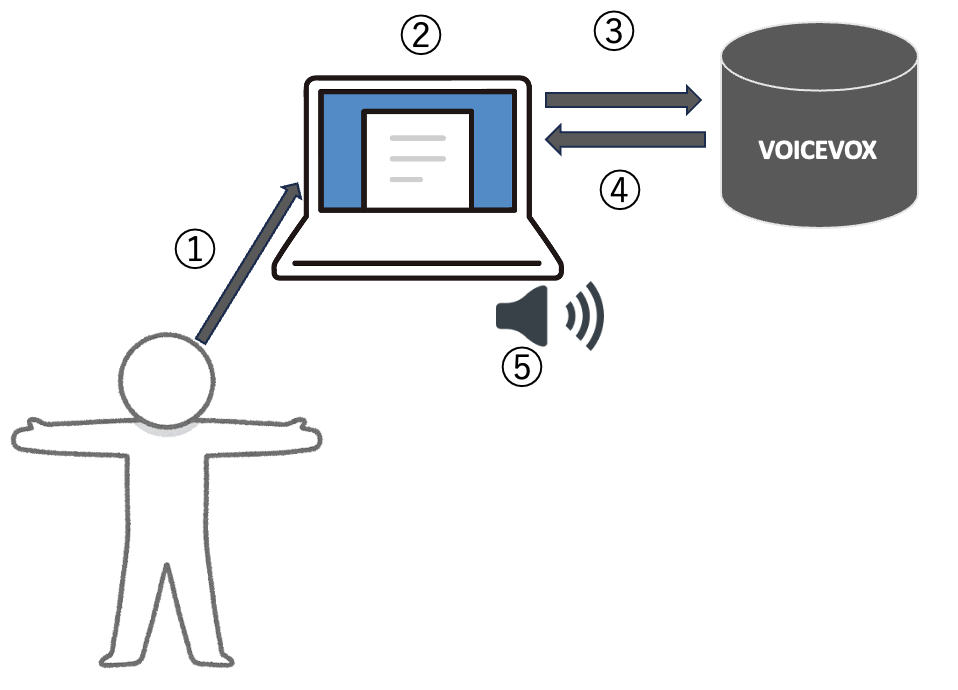
\includegraphics[width=7cm]{figures/system_figure.png}
      \caption{構成図}
      \label{fig:system_figure}
    \end{center}
  \end{figure}  

MediaPipe Pose\cite{mediapipe_pose_landmarker}はGoogleが開発した骨格推定ライブラリである。このライブラリにおいては、画像やビデオ内の人体のランドマークを検出することができる。
MediaPipe Poseではさまざまなモデルがあるが、今回使用したPose landmarker modelでは33点のランドマークを検出することができる。\ref{fig:mediapipe} に検出できるランドマークの例を示す。
\begin{figure}[H]
  \begin{center}
    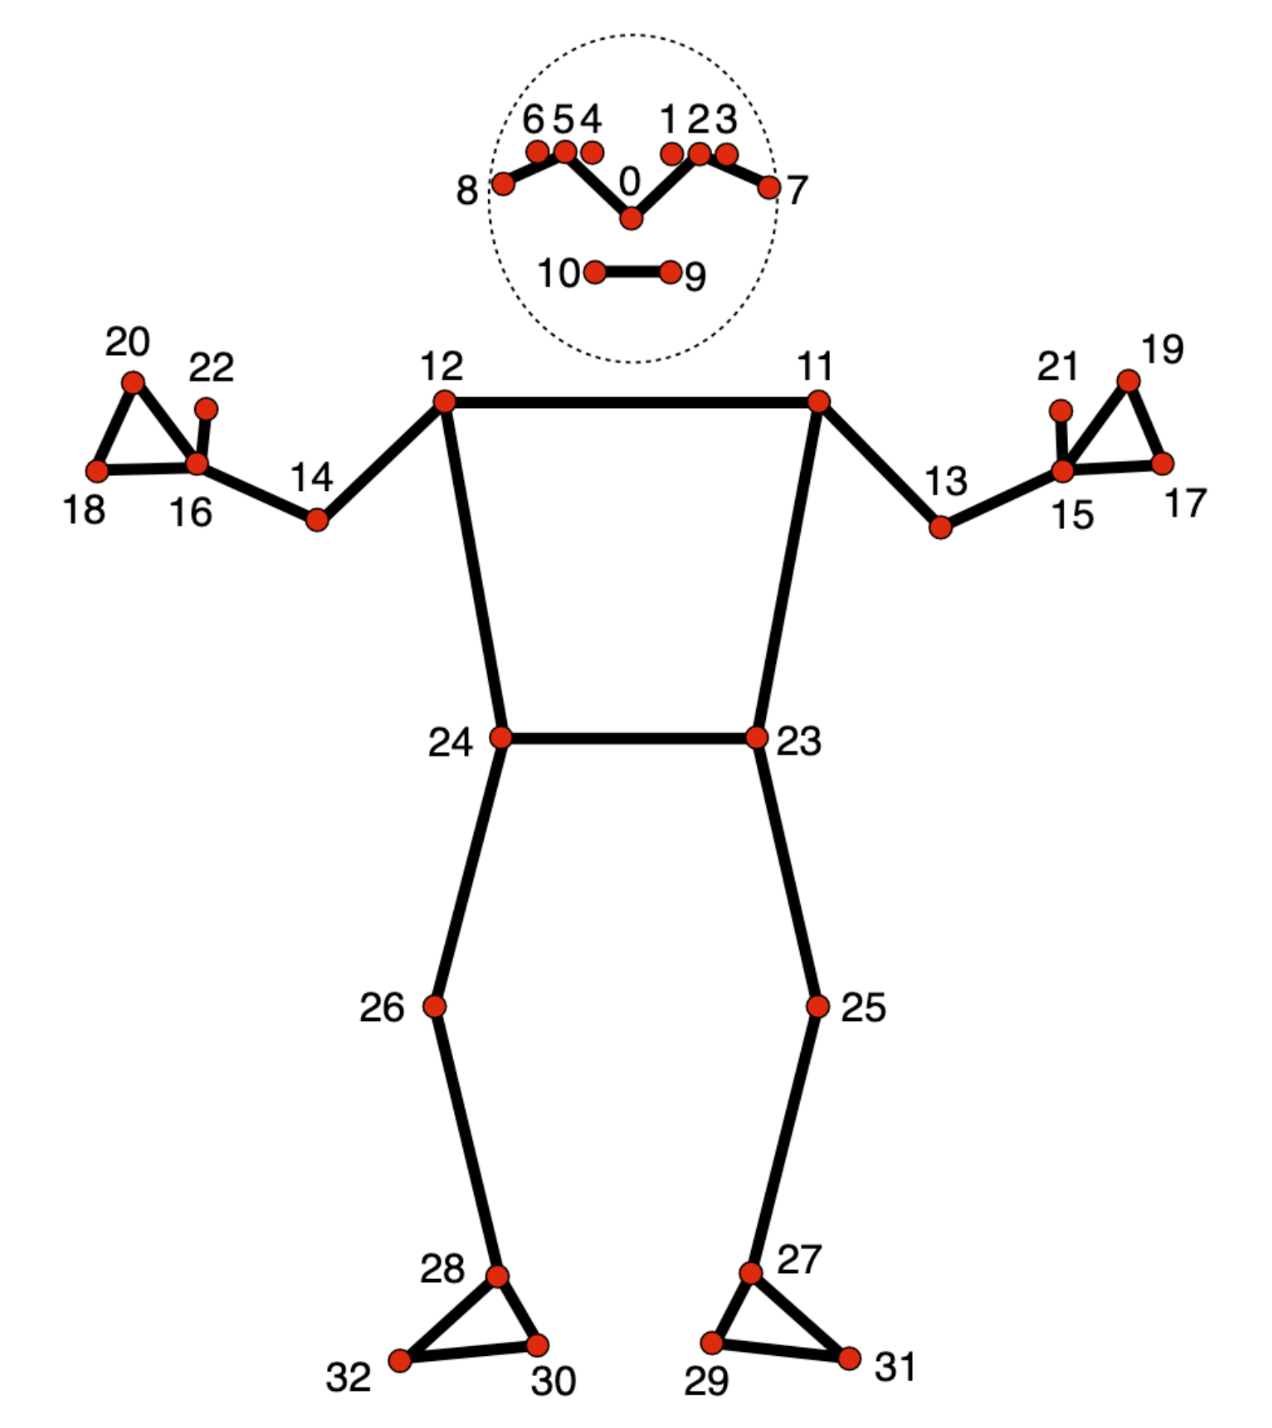
\includegraphics[width=7cm]{figures/mediapipe.png}
    \caption{MediaPipe Poseによるランドマークの検出ポイント}
    \label{fig:mediapipe}
  \end{center}
\end{figure}  
これにより、体の主要な位置を特定し、姿勢を分析し、動きを分類することが可能となる。単一の画像またはビデオを処理する機械学習モデルがこのライブラリで用いられる。
このライブラリを用いることで画像座標及び三次元世界座標における身体ポーズのランドマークを出力できる。
今回は手首(左右)、肘(左右)、肩(左右)のランドマークを検出し、肩、肘関節の角度について計測した。

VOICEVOXは商用・非商用問わず利用することができる無料で使える中品質なテキスト読み上げソフトウェアである。
今回はずんだもんの音声を使用した。
フィードバックとして与える言葉は以下の通りである。
\begin{enumerate}
  \item 右(左)肘を曲げてください
  \item 右(左)肘を伸ばしてください
  \item 右(左)腕を上げてください
  \item 右(左)腕を下げてください
\end{enumerate}
これらのフィードバックを関節角度に応じで読み上げる。

\subsection{デバイスとソフトウェア}
今回使用した環境は以下の通りである。
\begin{itemize}
  \item MacBook Pro (13-inch, M1, 2020)
  \item MacOS 13.5
  \item Python 3.8.12
  \item mediapipe 0.9.1.0
  \item numpy 1.23.5
  \item opencv-contrib-python 4.7.0.72
  \item VOICRVOX 0.14.10(ずんだもん)
\end{itemize}

